\begin{activity} \label{A:11.4.4} In this activity we determine integrals that represent the center of mass of a lamina $D$ described by the triangular region bounded by the $x$-axis and the lines $x = 1$ and $y = 2x$ in the first quadrant if the density at point $(x, y)$ is $\delta(x, y) = 6x + 6y + 6$. A picture of the lamina is shown in Figure \ref{F:11.4.COM_ex_1}.
\begin{figure}[ht]
\begin{center}
%\resizebox{!}{2.0in}{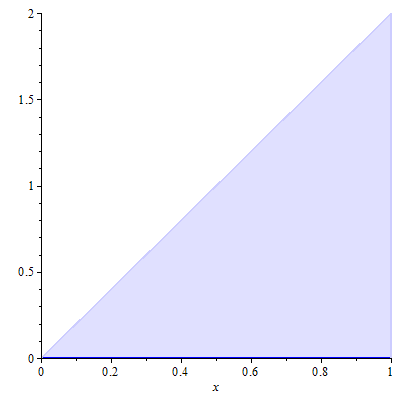
\includegraphics{11_4_COM_ex_1}}
  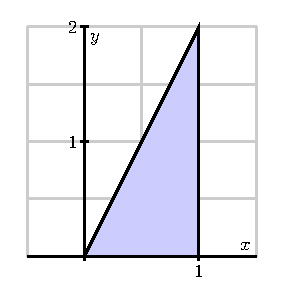
\includegraphics{figures/fig_11_4_triangle.eps}
\end{center}
\caption{The lamina bounded by the $x$-axis and the lines $x = 1$ and $y = 2x$ in the first quadrant.}
\label{F:11.4.COM_ex_1}
\end{figure}

    \ba
    \item Set up an iterated integral that represents the mass of the lamina.


    \item Assume the mass of the lamina is 14. Set up two iterated integrals that represent the coordinates of the center of mass of the lamina.


    \ea


\end{activity}
\begin{smallhint}

\end{smallhint}
\begin{bighint}

\end{bighint}
\begin{activitySolution}
\ba
\item The mass $M$ of the lamina is given by $\ds \int \int_D \delta(x,y) \, dA$. To calculate this mass, we set up an iterated integral, integrating first with respect to $y$ then $x$:
\[M = \int \int_D \delta(x,y) \, dA = \int_0^1 \int_0^{2x} (6x+6y+6) \, dy \, dx.\]
%\begin{align*}
%M &= \int \int_D \delta(x,y) \, dA \\	&= \int_0^1 \int_0^{2x} (6x+6y+6) \, dy \, dx \\
%	&= \int_0^1 \left[6xy+3y^2+6y\right]\biggm|_{0}^{2x} \, dx \\
%	&= \int_0^1 24x^2+12x \, dx \\
%	&= \left[8x^3+6x^2\right]\biggm|_0^1 \\
%	&= 14.
%\end{align*}

\item The $x$ coordinate of the center of mass is given by $\ds \frac{\int \int_D x \delta(x,y) \, dA}{14}$. An iterated integral that gives us this $x$ coordinate is 
\[\frac{1}{14}\int \int_D x \delta(x,y) \, dA = \frac{1}{14} \int_0^1 \int_0^{2x} x(6x+6y+6) \, dy \, dx.\]
%We need to evaluate the double integral
%$\ds \int \int_D x \delta(x,y) \, dA$ to complete this calculation:
%\begin{align*}
%\int \int_D x \delta(x,y) \, dA &= \int_0^1 \int_0^{2x} (6x^2+6xy+6x) \, dy \, dx \\
%	&= \int_0^1 \left[6x^2y+3xy^2+6xy\right]\biggm|_0^{2x} \, dx \\
%	&= \int_0^1 24x^3+12x^2 \, dx \\
%	&= \left[6x^4+4x^3\right]\biggm|_0^1 \\
%	&= 10.
%\end{align*}
%So the $x$ coordinate of the center of mass of the lamina is $\frac{10}{14} = \frac{5}{7}$.

The $y$ coordinate of the center of mass is given by $\ds \frac{\int \int_D y \delta(x,y) \, dA}{14}$. An iterated integral that gives us this $y$ coordinate is 
\[\frac{1}{14}\int \int_D y \delta(x,y) \, dA = \frac{1}{14} \int_0^1 \int_0^{2x} y(6x+6y+6) \, dy \, dx.\]
%We need to evaluate the double integral
%$\ds \int \int_D y \delta(x,y) \, dA$ to complete this calculation:
%\begin{align*}
%\int \int_D y \delta(x,y) \, dA &= \int_0^1 \int_0^{2x} (6xy+6y^2+6y) \, dy \, dx \\
%	&= \int_0^1 \left[3xy^2+2y^3+3y^2\right]\biggm|_0^{2x} \, dx \\
%	&= \int_0^1 28x^3+12x^2 \, dx \\
%	&= \left[7x^4+4x^3\right]\biggm|_0^1 \\
%	&= 11.
%\end{align*}
%So the $y$ coordinate of the center of mass of the lamina is $\frac{11}{14}$ and the center of mass of the lamina is $\left(\frac{5}{7}, \frac{11}{14}\right)$.
\ea

\end{activitySolution}
\aftera
